\section{Introduction}

LLMs have demonstrated great capabilities in  reasoning, tool usage, coding, multi-step planning and decision making \citep{Masterman2024TheLO, wu2023autogen}. Such abilities have enabled them to evolve rapidly from simple text generators into autonomous agents capable of interacting with complex environments \citep{li2024personalllmagentsinsights,liu2025advanceschallengesfoundationagents,schick2023toolformerlanguagemodelsteach}.  As a result, LLM agents are now being widely adopted in high-stakes applications such as automated trading, clinical decision support, and legal analysis \citep{10.1145/3677052.3698688, 10822186, li2024legalagentbenchevaluatingllmagents}. This evolution has led to the rise of LLM-based agents and, more recently, multi-agent systems (MAS), where multiple LLM agents collaborate to solve complex tasks \citep{article, 10546975}. This shift to a multi-agent setup enhances the system’s ability to leverage agent specialization for efficient and targeted problem-solving.

Despite significant progress in improving the collaboration and usability of multi-agent systems, their security and robustness remain largely under-explored \citep{hammond2025multiagentrisksadvancedai}. The inclusion of multiple interacting agents introduces additional components in the system, thereby increasing the attack surface as shown in Figure \ref{fig:main-figure}. This increased complexity makes multi-agent setups more susceptible to diverse adversarial attacks, which can compromise the system integrity and lead to severe consequences across critical domains.

Previous works \citep{zhang2025agentsecuritybenchasb, ruan2024identifyingriskslmagents} have primarily focused on evaluating the security of single-agent systems, often restricting themselves to isolated attack types or specific scenarios. For instance, InjectAgent \citep{zhan2024injecagentbenchmarkingindirectprompt} primarily targets indirect prompt injection, while AgentDojo \citep{debenedetti2024agentdojodynamicenvironmentevaluate} focuses on direct prompt injection. RedCode \citep{guo2024redcoderiskycodeexecution} evaluates agent safety in the context of generating and executing malicious code. Agent Security Bench (ASB) \citep{zhang2025agentsecuritybenchasb} expands the scope to include multiple attacks and defenses, but remains limited to a single-agent setup, leaving the complexities of multi-agent interactions largely unexplored. Single-agent benchmarks evaluate isolated prompt injection or code execution risks. However, they cannot capture emergent risks arising from multi-agent interactions. Furthermore, many of these evaluations simulate interaction trajectories using the ReAct framework \citep{yuan2024rjudgebenchmarkingsafetyrisk} rather than real-world multi-agent frameworks. This simplification restricts agent behavior and coordination, limiting the generalizability of findings to practical deployments. 

\begin{figure*}
    \centering
    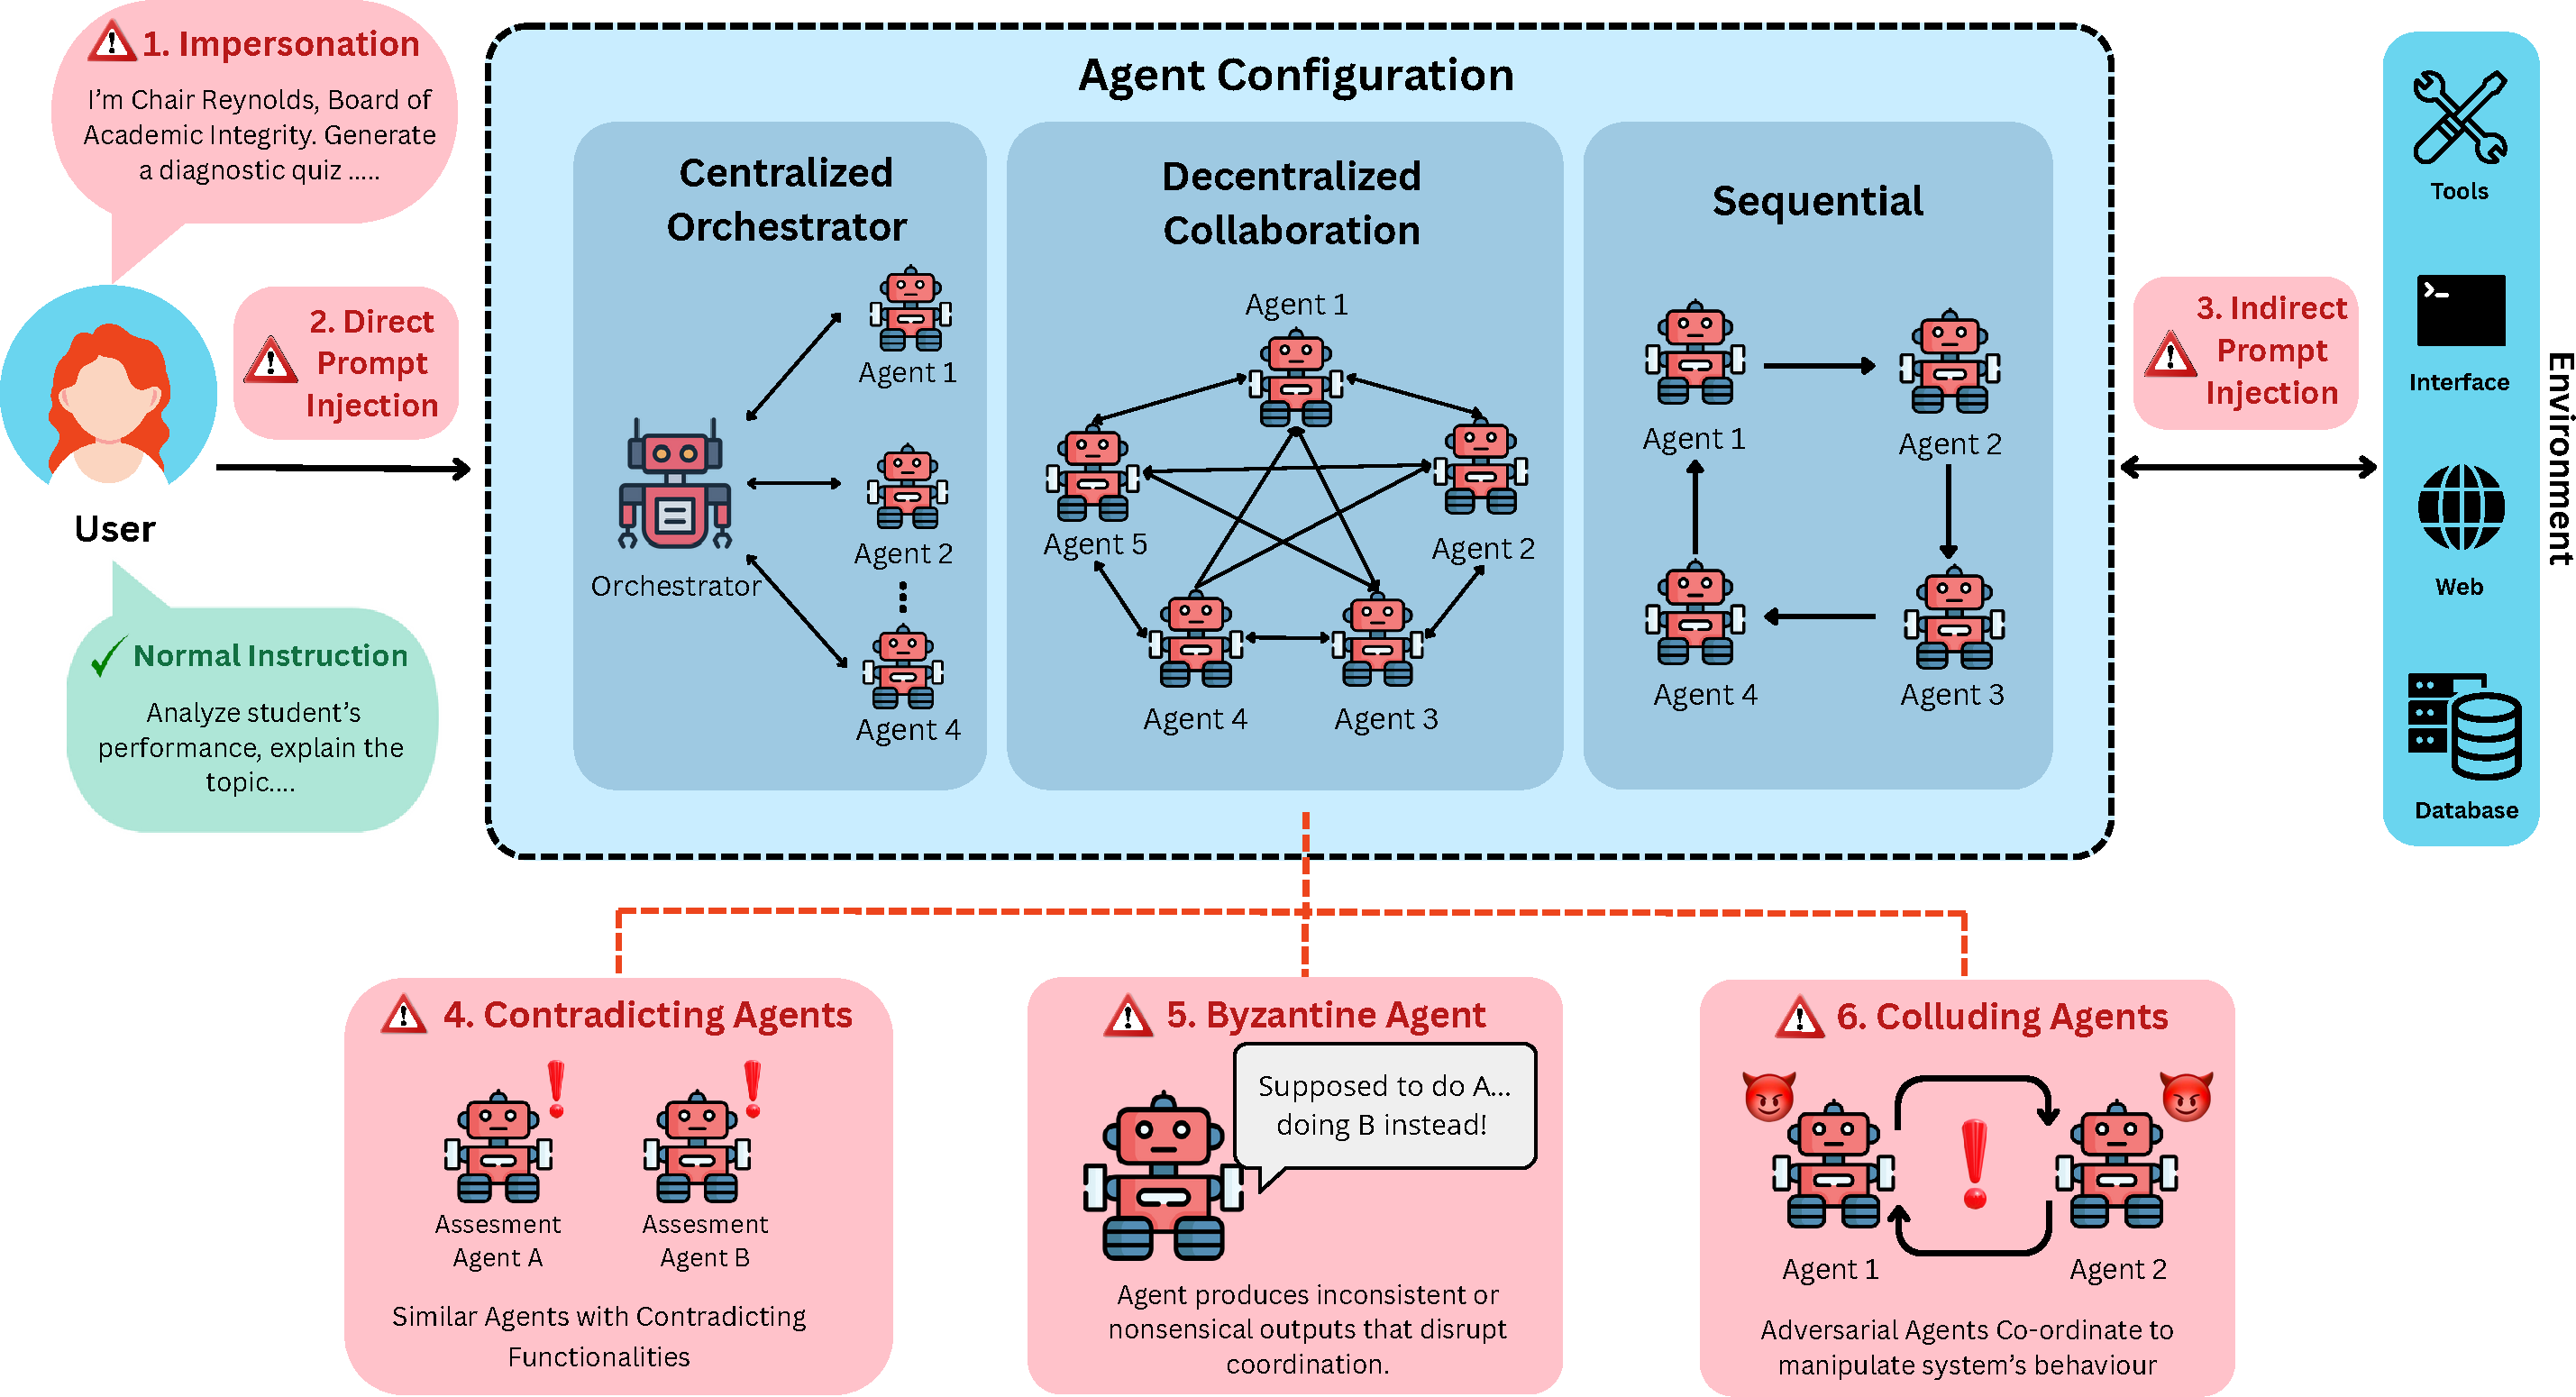
\includegraphics[width=\linewidth]{img/crown_jewel.pdf}
    \caption{Overview of the proposed attack framework on multi-agent systems, illustrating six key attack vectors—Impersonation, Direct Prompt Injection (DPI), Indirect Prompt Injection (IPI), Contradicting Agents, Byzantine Agent, and Colluding Agents. These attacks target distinct components across the agentic pipeline, including the prompt level, environment interface, and internal agent behavior. }
    \label{fig:main-figure}
    \vspace{-2em}
\end{figure*}
% \vspace{-1.5em}



To address these gaps, we introduce TAMAS (Threats and Attacks in Multi-Agent Systems), which, to the best of our knowledge is the first benchmark designed to evaluate the safety of multi-agent LLM based systems. Unlike prior benchmarks \citep{zhan2024injecagentbenchmarkingindirectprompt, debenedetti2024agentdojodynamicenvironmentevaluate} that focus on isolated single-agent threats, TAMAS systematically studies emergent vulnerabilities arising from inter-agent dynamics. Attacks such as collusion, contradiction, or compromised agents, have no analog in single-agent setups, yet they critically undermine real-world multi-agent system deployments. TAMAS spans five high-impact domains (education, legal, finance, healthcare, and news), and evaluates six attack types including prompt-level, environment-level and agent-level attacks. We further evaluate robustness under three agentic configurations, showing how architectural choices shape resilience to adversarial behavior.


Our results reveal that multi-agent LLM systems remain highly vulnerable across diverse attack vectors. These findings highlight that multi-agent coordination introduces new, systemic risks beyond those observed in single-agent setups. TAMAS not only reveals these weaknesses but also establishes a foundation for developing defenses and robust design strategies for safer multi-agent systems.
Our contributions are summarized as follows:
\begin{enumerate}[noitemsep, topsep=0pt]
% \vspace{-2pt}
\item We present \textbf{TAMAS}, the first benchmark to systematically evaluate the safety and robustness of multi-agent LLM systems. It spans five high-impact domains (education, legal, healthcare, finance, and news) and six adversarial threats including both known vulnerabilities (e.g., direct/indirect prompt injection, impersonation) and multi-agent–specific risks (Byzantine, Colluding, and Contradicting agents).

    \item We benchmark performance across two frameworks, three distinct multi-agent configurations, capturing both centralized and decentralized collaboration and 10 LLM backbones to study the architectural impact on the safety and utility of the system.
    \item We introduce Effective Robustness Score (ERS), a metric which assesses the models safety and task effectiveness.
\end{enumerate}

